\documentclass[12pt]{report}
\usepackage[pdftex]{graphicx}
\usepackage{url}
\usepackage{setspace}
\usepackage{makeidx}
\usepackage[utf8]{inputenc}
\usepackage{fancyhdr}
\usepackage{layout}
\usepackage{float}
\usepackage{titlesec}
\usepackage{graphicx}
\usepackage[a4paper,pdftex]{geometry}	% Use A4 paper margins
\usepackage[english]{babel}
\usepackage{xcolor} % Required for specifying custom colors
\usepackage{fix-cm} % Allows increasing the font size of specific fonts beyond LaTeX default specifications
\usepackage{amssymb}
\usepackage{amsthm}
\usepackage{amsmath}
\usepackage{hyperref}
\hypersetup{
    colorlinks,
    citecolor=black,
    filecolor=black,
    linkcolor=black,
    urlcolor=black
}

\DeclareGraphicsExtensions{.pdf,.png,.jpg}

\setlength{\oddsidemargin}{0mm} % Adjust margins to center the colored title box
\setlength{\evensidemargin}{0mm} % Margins on even pages - only necessary if adding more content to this template

\renewcommand{\thepart}{\arabic{part}}
\renewcommand{\thechapter}{\thepart.\arabic{chapter}}
\renewcommand{\thesection}{\thechapter.\arabic{section}} %Section numbering
\renewcommand{\thesubsection}{\thesection.\arabic{subsection}} %Subsection numbering

\setlength{\voffset}{-1.2cm}
\setlength{\textheight}{650pt}
\setlength{\parindent}{0pt}
\renewcommand{\baselinestretch}{1.5}
\definecolor{grey}{rgb}{0.95,0.95,0.95} % Color of the box surrounding the title - these values can be changed to give the box a different color	

\pagestyle{fancy}
\fancyhf{}
\lhead{A Fireball for Your Friends}
\rhead{Game Design Document: Part \thepart}
\rfoot{\thepage}

\newcommand*\cleartoleftpage{%
  \clearpage
  \ifodd\value{page}\hbox{}\newpage\fi
}

\newcommand{\sectionbreak}{\clearpage}

\makeindex

\begin{document}

\pagestyle{empty} % Remove page numbering on this page

%----------------------------------------------------------------------------------------
%	TITLE SECTION
%----------------------------------------------------------------------------------------

\colorbox{grey}{
	\parbox[t]{1.0\linewidth}{
		\fontsize{50pt}{30pt}\selectfont % The first argument for fontsize is the font size of the text and the second is the line spacing - you may need to play with these for your particular title
		\vspace*{0.7cm} % Space between the start of the title and the top of the grey box
		
		A Fireball \\ 
		for Your Friends \\ 
        \fontsize{30pt}{34pt}\selectfont
        Game Design Document		
		\par
		
		\vspace*{0.4cm} % Space between the end of the title and the bottom of the grey box
	}
}

\vspace*{0.4cm} 
{\large Un \textbf{juego de duelos mágicos multijugador en 3ª persona}}

\begin{spacing}{0.6}
Target: \textit{chicos entre 16-22 años, amantes de los juegos competitivos, mid-core} 

Plataforma: \textit{XBox One, Windows PC}
\end{spacing}


\begin{figure}[h]
    \centering
    \includegraphics[width=0.6\textwidth]{fireball}
\end{figure}

\vfill % Space between the title box and author information

{\centering \hfill \copyright 2018 Pedro Montoto García} \\

%----------------------------------------------------------------------------------------

\clearpage

\tableofcontents

\setlength{\voffset}{0cm}
\setlength{\parindent}{1cm}
\setcounter{page}{1}

\cleartoleftpage

\part{Game Overview}

\chapter{General Characteristics}

\section{High Level Concept}
\pagestyle{fancy}

Un juego multijugador\footnote{Este documento se incluye como anexo a un \textit{vertical slice} del juego descrito por el propio documento, que ejemplifica la experiencia de un modo de juego de combate de dos jugadores (uno de los cuales es manejado por la IA). Todas las features implementadas en dicho \textit{vertical slice} se indican como tales en sus respectivas secciones.} (pantalla partida y online) en tercera persona donde dos equipos cada uno con de 1 a 3 magos duelean en un pequeño escenario usando hechizos variados y espectaculares. Cada jugador deberá componer su biblioteca de hechizos en cada encuentro, escogiéndolos según la utilidad que tengan para contrarrestar al enemigo y sinergizar con sus aliados.

Cada encuentro tendrá sus objetivos, i.e. aniquilación, capturar la bandera, defender un objetivo, football (à la Rocket League)..., y su duración será corta, i.e. entre 5 y 10 minutos, para asegurar que todo el mundo pueda disfrutar de al menos una partida rápida, pero que ésta sea intensa. Podemos describir este juego en términos de ``ajedrez a la velocidad de la luz''.

La experiencia de juego se centra en hacer que el jugador sienta su maestría al derrotar a enemigos usando los diferentes hechizos, evitándolos a su vez. El loop de juego principal estará en dominar los diferentes hechizos y sus sinergias via el empoderamiento del jugador.

\begin{figure}[h]
    \centering
    \includegraphics[width=0.8\textwidth]{tf2}
    \caption{Tomamos de Team Fortress 2 la variedad de gameplay, la velocidad de la acción y lo intuitivo que resulta para nuevos jugadores}
\end{figure}

\section{State of the Art}

\subsection{Competitors}
Este juego compite directamente con otros shooters multijugador competitivos como \textit{Call of Duty}, \textit{Battlefield}, \textit{PlayerUnknown's BattleGrounds (PUBG)} (éste en 3ª persona también), \textit{Counter Strike} etc. También entra en el mercado de los Multiplayer Online Battle Arena (MOBAs) y otros tipos de videojuego altamente competitivos, como \textit{Defense of the Ancients (DOTA)} y \textit{League of Legends (LOL)}. Dado que la temática es mágica-medieval y adulta también podría ocupar espacio de mercado de juegos de fantasía altamente centrados en gameplay en 3ª persona (con un multiplayer altamente competitivo) como la saga \textit{Dark Souls}.

\subsection{Overcoming Competitors: Unique Selling Points}
Para convencer a la gente que está jugando los juegos arriba mencionados optaremos por aprovechar:

\begin{itemize}
\item La combinación de shooter altamente competitivo con una ambientación fantástica, que no ha sido probada aún en el mercado.
\item Gameplay sólido con control altamente responsivo
\item Situaciones espectaculares que hacen fácil que el juego se promocione a sí mismo en redes sociales, mediante el reenvío de gifs o vídeos con jugadas llamativas
\item Personalización en todos los aspectos del juego (desde habilidades hasta apariencia)
\end{itemize}

\section{Visual Appeal}

\subsection{Character appeal}

Dado que no planteamos un modo historia de un sólo jugador, sino que la historia se ve símplemente como un extra que añade una capa de profundidad al modo multijugador como flavor text de hechizos y personalizaciones, en este apartado nos centraremos en conseguir una estética agradable, personal y que envejezca bien (i.e. Team Fortress, Overwatch) dado que siendo multijugador nuestro planteamiento es alargar la vida del juego lo máximo posible. Por tanto, para ello se utilizarán gráficos estilizados y simplificados adornados por gran variedad de efectos.

Otro punto importante en los gráficos es la variedad de elementos de personalización del personaje jugador, de los entornos y de los efectos de hechizo.

\subsection{Scope of Visual Effects: Visual Variety}

Estamos orientados a hacer este juego lo más espectacular y variado posible. Siendo la variedad de hechizos uno de nuestros Unique Selling Points haremos cada hechizo fácilmente reconocible por sus efectos visuales al mismo tiempo que las combinaciones que cada jugador escogerá en sus partidas sean únicas en cada una. Para conseguir ésto se utilizará todo el potencial de efectos especiales, efectos de partículas y post-procesado de pantalla completa.

\subsection{Environment Appeal}

Los entornos serán simples pero rápidamente identificables. La idea es que los entornos sirvan para aumentar la variedad de situaciones que el jugador afrontará durante sus partidas: aunque se ponga la atención en su atractivo visual éste no es el objetivo principal de nuestros entornos de juego.

\section{Gameplay Features}     

\subsection{Reward systems}

\begin{itemize}
\item Un sistema de desbloqueo de habilidades irá guiando al jugador de hechizos más simples a otros más complejos, para que su curva de aprendizaje sea menos costosa. Sistemas similares se usan en Heroes of the Storm y LOL, o el modo ``héroes simples'' en DOTA.
\item Como extensión del sistema previo, un subsistema de niveles y puntos de experiencia por partida finalizada recompensará al jugador con sistemas de personalización variados. Se establecerán quests diarias con recompensas de experiencia extras para recompensar a los jugadores que asisten al juego más regularmente.
\item Un modo de juego competitivo, desbloqueable para jugadores con experiencia por encima de lo que consideremos \textit{niveles de tutorial}, proveerá a los jugadores más hardcore de un modo de juego más acorde a sus gustos.
\end{itemize}     

\subsection{Modes of play}

El modo básico de juego es el multijugador, que permite a cada jugador conectarse a un servidor central de lobbying de partidas y jugar con sus amigos o desconocidos a través de internet. El juego también permite a jugadores juntarse en una casa, conectar la Nintendo Switch y jugar en pantalla partida compartiendo un televisor. Los jugadores pueden loguearse en sus propias cuentas y usarlas en la consola de un amigo o bien usar una copia del personaje del dueño de la consola con colores cambiados.

El juego ofrece un modo de práctica contra maniquíes de mago, para probar y practicar habilidades \footnote{En esto consiste el \textit{Vertical Slice}.}. El core del juego será la elección de ``modo de dificultad'' multijugador:

\begin{description}
\item[Quick Play:] Modo ``Casual'' de partidas rápidas
\item[Competitivo:] Modo ``Serio'' donde se asume mayor habilidad y coordinación dentro del equipo
\end{description}

En Quick Play o Competitivo pueden jugarse los siguientes modos:

\begin{description}
\item[Exterminación:] \textit{Implementado en el Vertical Slice}, 1v1 contra IA. Equipos de Magos intentan matarse unos a otros con un límite de tiempo. Gana el equipo que tenga más componentes vivos al final del límite de tiempo o que consiga matar a todos los enemigos dentro de dicho límite.
\item[Capturar la Bandera:] Existen bases para cada equipo y cada una guarda una bandera. El objetivo es entrar en la base enemiga y llevar la bandera enemiga a la base propia. Gana el equipo que más puntos tenga al final del límite de tiempo.
\item[Football:] El entorno de juego es un campo libre con dos ``porterías'' en los extremos, cada una de un equipo. El modo de juego consiste en combinar la lucha con el uso de los hechizos para meter la pelota en la portería contraria. Gana el equipo que más goles tenga al final del límite de tiempo.
\item[King of the Hill:] Se designa una zona especial de captura en el mapa, con un tiempo límite para cada equipo. El tiempo límite de cada equipo desciende hacia 0 mientras la zona de captura está en sus manos. Gana el primer equipo que lleve a 0 su contador de tiempo límite.
\end{description}

\cleartoleftpage

\part{Gameplay}

\chapter{User Interaction Elements}

En éste capítulo\footnote{El contenido de esta parte está explicado tal cual aparece en el \textit{vertical slice}, a menos que se indique lo contrario.} describiremos primero la representación en UI + Controles de las posibles acciones del jugador para pasar luego, en el siguiente capítulo, a los sistemas que soportan la interacción del jugador. Todos los datos necesarios para el funcionamiento de la interfaz, incluídos los hechizos, se construyen proceduralmente sobre dichos sistemas, permitiendo la iteración rápida. Si algún elemento no dependiese directamente de algún subsistema de gameplay (i.e. es pura representación para el jugador), se describe en éste capítulo.

\section{Control}

El jugador puede realizar las siguientes acciones, que se describen a continuación:

\begin{itemize}
	\item Moverse + Saltar
	\item Fijar la cámara en el enemigo ó Mover la cámara libremente (autoapuntado vs apuntado libre)
	\item Disparar un hechizo ó Cambiar el hechizo seleccionado
	\item Usar un hechizo de utilidad (Un escudo mágico, p.ej.)
\end{itemize}

En las siguientes secciones se describen los controles que ejecutan estos verbos y cómo se realizan en concreto, a nivel de diseño y motor de juego (Unreal).

\section{Controller Config}
\label{control1}

Se recomienda jugar con un mando estilo XBox (360 / One) y la siguiente configuración, incluída por defecto en el \textit{vertical slice}.

\begin{figure}[h]
    \centering
    \includegraphics[width=0.8\textwidth]{controller}
    \caption{El control deberá ser completamente configurable, con estos valores por defecto en juego}
\end{figure}

Se trata de una configuración que cumple las convenciones del género (shooter en 3ª persona) para movimiento, cámara y disparos, añadiendo los controles que hacen diferente al juego (selección de objetivos) en los botones que quedan libres.

\section{Keyboard + Mouse Config}
\label{control2}

En caso de no haber controlador XBox o similar disponible puede recurrirse al control mediante teclado y ratón, que diverge del control con mando únicamente al no estar disponible el \textit{force feedback}.

\begin{figure}[h]
    \centering
    \includegraphics[width=\textwidth]{keyboard}
\end{figure}

Al igual que el esquema de control sobre mando se han usado las convenciones del género, cambiando el control usual para cambio de arma (barra de números en el teclado, sobre WASD) y reinterpretándolo como ``cambio de hechizo''.

\section{User Interface}

Para explicar los elementos de la interfaz de usuario nos basaremos en la siguiente captura de pantalla del prototipo, al que se le ha aplicado un efecto de post-procesado que divide la pantalla en 10 cuadrantes horizontal y verticalmente, lo que nos permite ver mejor el posicionamiento y proporciones de los elementos. El jugador se posiciona respecto a la cámara en el 5º cuadrante desde la izquierda y entre el 7º y 10º cuadrantes desde arriba. Esto se hace así para dejar ver lo que se está apuntando en cada momento exactamente en el centro de la pantalla.

\begin{figure}[h]
    \centering
    \includegraphics[width=\textwidth]{UI_Example}
\end{figure}

\begin{figure}[h]
    \centering
    \includegraphics[width=0.5\textwidth]{camera_position_presets}
    \caption{Posicionamiento de la cámara respecto al jugador}
\end{figure}

\begin{figure}[b]
    \centering
    \includegraphics[width=1\textwidth]{alignments}
    \caption{Vemos aquí el alineamiento entre los diferentes elementos de la UI}
\end{figure}

\subsection{Life and Mana Bars}

\begin{figure}[H]
    \centering
    \includegraphics[width=1\textwidth]{life_mana_bars}
    \caption{Las barras de vida y maná muestran el descenso gradual mientras se usan los respectivos recursos (explicados más adelante) e incluyen la cifra exacta (actual / máximo) para que el jugador pueda ver con exactitud cuánto tiene de cada recurso.}
\end{figure}

\subsection{Aiming Crosshairs}

\begin{figure}[H]
    \centering
    \includegraphics[width=\textwidth]{crosshairs}
\end{figure}

Como se puede ver, la UI incluye 2 retículas de apuntado representadas como círculos mágicos (resaltadas en negro aquí). La retícula pequeña a la derecha, la retícula de \textit{apuntado real}, se sitúa siempre en el centro de la pantalla, señalando la posición de encarado y apuntado. La grande a la izquierda, la retícula de \textit{autoapuntado}:

\begin{itemize}
	\item \textbf{En modo de autoapuntado} señala el objetivo fijado por los controles situando su centro sobre el objetivo, la retícula de \textit{apuntado real} se mueve siempre hacia ella, centrándose perfectamente en el momento en que se intenta lanzar un hechizo de ataque. \textbf{En modo de apuntado libre} la retícula permanece concéntrica con la retícula de \textit{apuntado real}.
	\item Realiza un efecto de ``acelerado y tensado (encogimiento)'' sobre el objetivo mientras se está preparando un hechizo, para comunicar la tensión aumentada del fijado de objetivo al intentar lanzar un hechizo sobre él.
	\item Refleja la distancia al objetivo haciéndose más grande o más pequeña según la posición relativa del jugador y el objetivo.
\end{itemize}

Los detalles de éste elemento se controlan, animados por el parámetro \textit{FocusAlpha} desde \textit{\emph{MainPlayerBP}}, con los parámetros de la clase \textit{\emph{BaseMagicCrosshairBP}}. Parámetros de animación:

\begin{description}
	\item[FocusAlpha] Float. Este parámetro controla la \textit{concentración} del propietario de la retícula, y es responsabilidad del objeto propietario animarla. El valor tiene sentido entre 0 y 1 ambos inclusive, y sirve para interpolar linealmente entre los siguientes pares de valores.
	\item[ScaleAtMin/MaxFocus] Vectores 3D. Estos parámetros controlan lo grande o pequeña que la retícula se hace según la cantidad de focus. La intención es que a mayor focus más pequeña (centrada) es la retícula correspondiente.
    \begin{align}
		ScaleAtMinFocus &= [1.0, 1.0, 1.0] \\
		ScaleAtMaxFocus &= [1.0, 0.7, 0.7]
   	\end{align}
	\item[RotationSpeedAtMin/MaxFocus] Vectores 3D Rotator. Estos parámetros controlan lo rápido que gira la retícula según la cantidad de focus. La intención es que a mayor focus más rápido gira la retícula correspondiente.
    \begin{align}
		RotationSpeedAtMinFocus &= [ 90º/s, 0.0, 0.0] \\
		RotationSpeedAtMaxFocus &= [720º/s, 0.0, 0.0]
   	\end{align}
\end{description}

Parámetros de movimiento respecto a objetivo:

\begin{description}
	\item[Target] Tipo \textit{\emph{TargetableBPInterface}}\footnote{Descrito en los sistemas de gestión de hechizos, más adelante. Por el momento, para éste subsistema, representa la posición del objetivo fijado.}. Este parámetro representa el objetivo fijado por el jugador (en el modo de autoapuntado) o la posición del elemento que el jugador tenga exactamente en frente (en el modo de libre apuntado).
	\item[ConvergenceRate] Float. Este parámetro regula el ratio de convergencia entre 2 valores que dependan de la posición relativa entre el propietario de las retículas y el objetivo, por ejemplo la posición de la retícula entre ambos, siendo 0 el valor de convergencia nula y 1 el valor de convergencia instantánea. Este parámetro se utiliza para suavizar transiciones abruptas como las existentes entre los cambios de modo de control, que mueven el parámetro \textit{Target} bruscamente (i.e. entre la posición del enemigo seleccionado y lo que el jugador tenga exactamente en frente). Animado dentro del propio \textit{\emph{BaseMagicCrosshairBP}}.
	\item[ProportionOfDistanceToEnemy] Float. Este parámetro regula, dentro de la distancia que separa a la raíz de la retícula y el objetivo, dónde debe situarse en tamaño la retícula. Valores sensatos entre 0 y 1: fuera de éste rango, debajo de 0 significa ``detrás de la raíz de la retícula'' y por encima de 1 ``por detrás del objetivo actual''.
    \begin{align}
		ProportionOfDistanceToEnemy &= 0.2
   	\end{align}
\end{description}

\subsection{Spell Info}

A continuación describimos la interfaz que representa los hechizos seleccionados y su estado. Se puede ver que cada icono, representando los poderes de dicho hechizo, incluye información sobre su \textit{coste en maná} y su \textit{cooldown restante}\footnote{El sistema de magia se describe más adelante.} (como una barra que se descarga hasta que el hechizo vuelve a estar preparada para usarse), además del botón que sirve para seleccionarlo. Incluímos además una barra de color dorado alrededor del hechizo seleccionado en cada momento. 

\begin{figure}[H]
    \centering
    \includegraphics[width=0.5\textwidth]{magic_ui}
    \caption{La colección de hechizos presente en este momento}
\end{figure}

\begin{figure}[H]
    \centering
    \includegraphics[width=0.5\textwidth]{magic_utility_ui}
    \caption{El hechizo de utilidad seleccionado. Dicho hechizo funciona exactamente igual que cualquier otro hechizo del juego, pero está asociado a un control diferente que hace que esté siempre disponible para uso directo con un sólo botón.}
\end{figure}

\chapter{Game Systems}

\section{Movement Design}

Todo movimiento se realiza relativo a la transformación de la cámara, siendo ``adelante, derecha y arriba (salto)'' los movimientos básicos, interpretados relativamente a la cámara, sobre los que se compone el movimiento final. El movimiento se considera como absoluto respecto a la cápsula que contiene al personaje: cualquier movimiento extra (i.e. encarado del personaje) es símplemente una representación visual para mejorar el \textit{Game Feel}, codificada en el Animation Blueprint del personaje, que no tiene efecto real a nivel de gameplay.

El movimiento está diseñado para proporcionar una respuesta inmediata y consistente en todo momento: el jugador ha de sentirse en control. Para ello el jugador siempre se mueve a velocidad máxima y sin tener que esperar para girarse. Su zona de control tiene por tanto esta forma:

\begin{figure}[H]
    \centering
    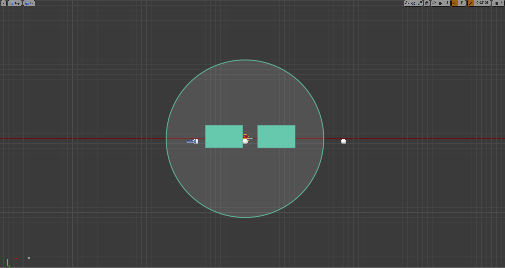
\includegraphics[width=0.8\textwidth]{movement}
\end{figure}

Se ha proporcionado la habilidad de salto para poder acceder a escenarios con diferentes alturas y dar al jugador una válvula de escape ante enemigos que puedan atosigarlo con múltiples proyectiles. El salto añade un movimiento repentino hacia arriba que hace posible esquivar proyectiles rápidos. 

\begin{figure}[H]
    \centering
    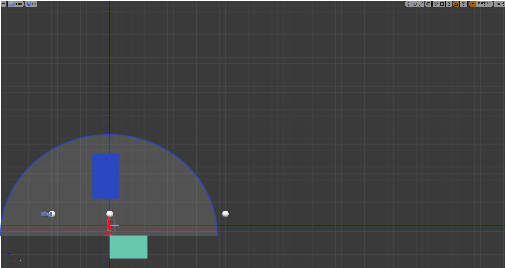
\includegraphics[width=0.8\textwidth]{movement_jump}
\end{figure}

El jugador puede moverse y cambiar de dirección instantáneamente a la misma velocidad que si estuviese en el suelo, por tanto tiene la misma zona de control horizontal en salto o moviéndose por el suelo. Se utiliza la gravedad por defecto de Unreal.

\section{Resource System}

\begin{figure}[H]
    \centering
    \includegraphics[width=1\textwidth]{resources_diagram}
\end{figure}

Definimos un recurso como una cantidad (float) que puede gastarse mientras esté sobre 0 y que tiene un máximo que puede almacenarse. La cualidad y comportamiento de \textit{ser un recurso} está definida en la interfaz \textit{\emph{ResourceBPInterface}} y el comportamiento básico de todos los recursos del juego queda descrito en el componente \textit{\emph{ResourceManagerCBP}}. Esta clase general nos permite modelar cualquier comportamiento que pueda tener un recurso derivándola a clases hijas con comportamientos más específicos, de ser necesario.

Un recurso tiene los siguientes parámetros:

\begin{description}
	\item[Max] Float. La cantidad máxima de recurso que se puede acumular.
	\item[Current] Float. La cantidad actual de recurso que el actor que posee el componente tiene.
\end{description}

Y los siguientes comportamientos, derivados de la interfaz:

\begin{description}
	\item[Refill()] Rellena el valor \textit{Current} del recurso hasta \textit{Max}.
	\item[Earn(Amount:Float)] Rellena el valor \textit{Current} en \textit{Amount} unidades sin sobrepasar \textit{Max}.
	\item[CanSpend(Amount:Float)] Devuelve un valor booleano \textit{True} si la cantidad especificada \textit{Amount} es mayor que la cantidad \textit{Current} de recurso, \textit{False} en caso contrario.
	\item[Spend(Amount:Float, Force: Boolean)] Decrementa \textit{Current} en \textit{Amount} unidades si \textit{CanSpend(Amount)} es \textit{True}. El parámetro \textit{Force} permite gastar dicha cantidad aunque \textit{CanSpend(Amount)} sea \textit{False} (dejando \textit{Current} en negativo).
\end{description}

\subsection{Health System}

El sistema de salud se basa en un recurso, implementado en \textit{\emph{HealthManagerCBP}}, que para ser más fácilmente identificable implementa la interfaz \textit{\emph{DamageableBPInterface}}\footnote{Esta misma interfaz es implementada por los jugadores y cualquier elemento que sea dañable. En el caso de los jugadores la implementación delega en un HealthManagerCBP su funcionamiento, después de generar los efectos de feedback al jugador dentro de su propia implementación. Al tener jugadores y componente la misma interfaz conectarlos es trivial.} y delega las funciones ReceiveDamage y WillDieIfDamaged al sistema de recursos.

El recurso pone a disposición del usuario 2 eventos que nos permiten implementar comportamiento relativo a ellos en otros Blueprints:

\begin{description}
	\item[OnDamageReceived] Se lanza este evento siempre que se llame a ReceiveDamage(), inmediatamente después de aplicar los efectos del daño.
	\item[OnDie] Si el resultado de ReceiveDamage() resulta en la muerte del jugador ($Current <= 0$), se lanza este evento inmediatamente después de aplicar los efectos del daño.
\end{description}

\subsection{Mana System}

De forma similar al sistema de salud, el sistema de Maná en \textit{\emph{ManaManagerCBP}} implementa su propia interfaz que nos permite diferenciar actores que usan maná, como los jugadores. No implementa eventos propios, aunque en futuras iteraciones puede seguirse esta estrategia para acoplar efectos a los gastos y recuperaciones de maná. Sí implementa un atributo propio:

\begin{description}
	\item[ManaRechargePerSecond] Float. La cantidad de maná que se recupera por segundo, gestionado en el \textit{Event Tick} del componente.
\end{description}

\section{Magic System} 

\section{Game Structure}              

\subsection{Tutorial and training}

TBD

Se diseña un nivel de tutorial (ver abajo) en el que el jugador aprenderá los hechizos básicos: la Bola de Fuego, el Escudo Reflector y Cura guiado por un narrador. Una vez el jugador haya superado o rechazado jugar este nivel de tutorial se le permitirá entrar en el modo online y adquirir nuevas habilidades que podrá probar dentro del mismo nivel de tutorial.

\subsection{Accessibility}

Un modo gráfico extra adapta la visibilidad de pantalla para personas con daltonismo.

\subsection{Level Design}

El diseño de los niveles es minimalista y simplificado, para dejar paso a gameplay emergente dadas las habilidades y movimientos de los participantes. Se presenta aquí el diseño básico de un nivel del modo tutorial y otro nivel del modo Capturar la Bandera.

\begin{figure}[H]
    \centering
    \includegraphics[width=0.8\textwidth]{tutorial}
    \caption{Un nivel de tutorial}
\end{figure}


\begin{figure}[H]
    \centering
    \includegraphics[width=0.7\textwidth]{flags}
    \caption{Un nivel de CTF. Las X representan banderas y los círculos son coberturas destructibles.}
\end{figure}

\cleartoleftpage

\part{External Technical Details}

\section{Monetization: Game Life Cycle}

La esperanza de vida del juego queda definida como 10.000 jugadores online diarios, ó 7 jugadores concurrentes buscando partida por minuto, ó 1 partida formándose por minuto. Llegado este punto el juego online es claramente insostenible (demasiado tiempo de espera por una partida). Todo plan de negocio planteado para este juego ha de tener este dato en cuenta. Para ello el juego debe ser constantemente rejugable y por tanto han de incluírse quests diarias para reclamar la atención regular del jugador combinado con un gameplay ajustado y dinámico.

Todos los datos de juego (desbloqueos y personalización) se guardan en un sistema de servidores remoto que será accedido por el juego para matchmaking, esto aumenta los costes de mantenimiento del producto. Para costearlos se plantea un flujo de insumos proveniente de la venta de \textit{lootboxes} con contenido estético y nuevos elementos de jugabilidad (hechizos) para los personajes. A largo plazo puede extenderse a nuevos modos de juego o incluso campañas con foco narrativo que extiendan el universo de juego.

\section{Network}

Para garantizar la mejor experiencia de usuario a un coste bajo se utiliza una combinación de servicios mínimos para dar la información mínima a los clientes de juego para que gestionen partidas entre ellos, enviando de vuelta al servidor cada uno su copia local de la partida jugada para valoración anti-cheat. Como ejemplo, \textit{Raiders of the Broken Planet} utiliza un sistema de matchmaking similar a éste, siendo necesario el trabajo de matchmaking cross-platform para mantener unos niveles de jugadores concurrentes aceptables (para tiempos de matchmaking bajo).

\begin{figure}[h]
    \centering
    \includegraphics[width=0.6\textwidth]{network}
\end{figure}

\cleardoublepage

\thispagestyle{empty}

\vspace*{\fill}

\begin{figure}[h]
    \centering
    \includegraphics[width=0.6\textwidth]{fireball}
\end{figure}

\vfill

\end{document}
